\section{Tests et exemple}
\subsection{Test unitaire}

Consigne : description des tests, discussion de leurs résultats, explication des problèmes, des défauts et bugs. Pour chacun des tests avec : (1) spécification et buts du test ;
(2) cas de tests (données) utilisé ; (3) scénario du test ; (4) analyse du test et les moyens de mise en œuvre de cette analyse.

\begin{itemize}
    \item Il ne faut pas qu'un utilisateur puisse lancer une nouvelle partie sans finir la partie courante. Il faut tester à chaque nouvelle partie si l'utilisateur ne participe pas dans une partie déjà existante. Si c'est le cas, alors refuser la partie.
    \item Tester si une partie est finie, si toutes les conditions sont atteintes. Dans notre cas on va simplifier le scénario et considérer que la partie est finie quand la base principale est prise. La perte de celle-ci doit finir la partie et afficher le joueur gagnant.
    \item \lstinline{Mocha}, un framework qui permet de réaliser des tests de fonctionnement de nos fonctions. Nous créons un fichier dans le chemin :\href{https://gitlab.emi.u-bordeaux.fr/vsamson/desert-fox/-/blob/main/src/backend/src/test/index.test.ts}{index.test.ts}, il permet de vérifier le(s) erreur(s) dans les fonctions qu'on a pushé et on pourra vérifier dans les \href{https://gitlab.emi.u-bordeaux.fr/vsamson/desert-fox/-/pipelines}{pipelines}.
          %item test système :

          %\item tests  serveur
          %\item tests des besoins :
          %\begin{itemize}
          %    \item test des besoins fonctionnel :
          %    \item test des besoins non-fonctionnel :
          %\end{itemize}

\end{itemize}

\subsection{Couverture du code}

Le framework \lstinline{NYC} nous permet de tester la couverture. Il faut lancer la commande \emph{yarn test} dans le \lstinline{backend} ce qui créé dans le dossier \lstinline{coverage} où se trouve à l'intérieur un \lstinline{index.html} qui donne ceci.

\begin{figure}[H]
    \centering
    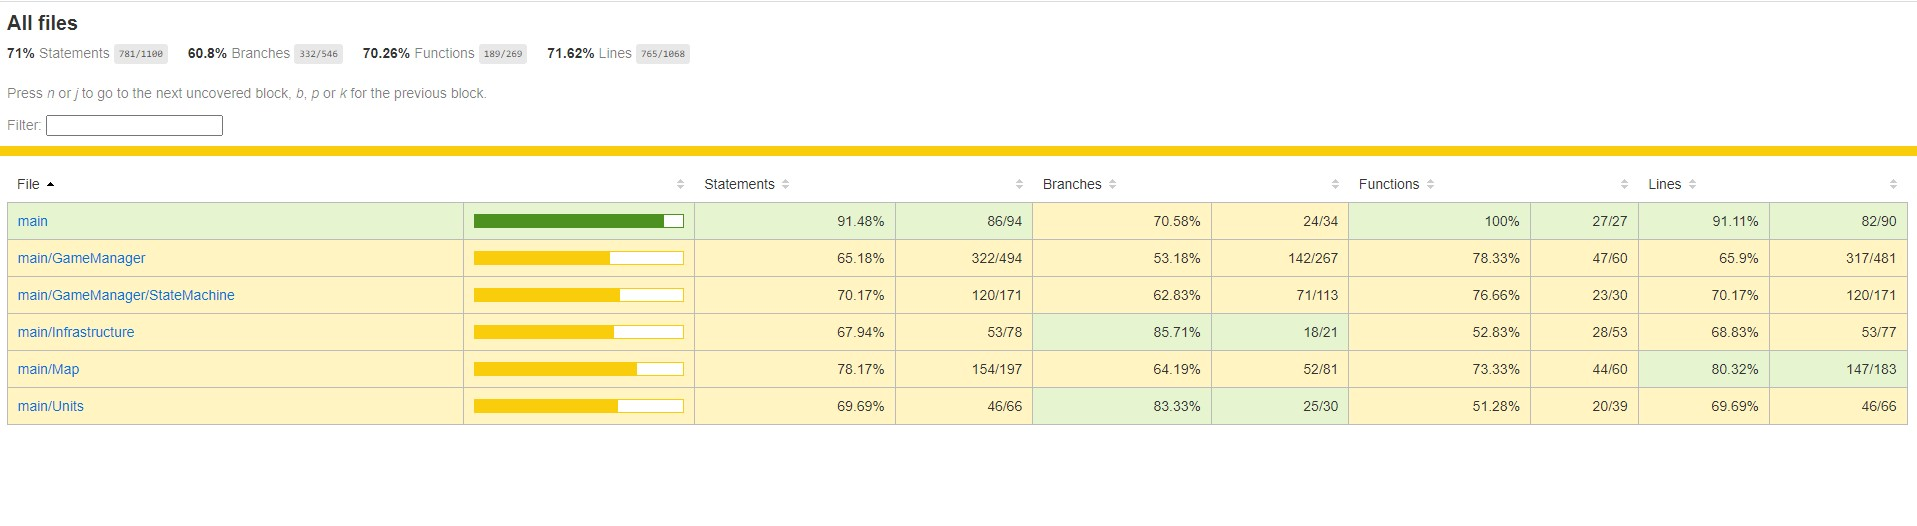
\includegraphics[scale=0.35]{data/couverture_test_1.jpg}
    \caption{Couverture générale du backend}
\end{figure}

On peut voir le pourcentage de couverture de chaque fichier. On peut aussi aller plus dans les détails et regarder ligne par ligne pour être sûr qu'absolument tout le code soit testé.

\begin{figure}[H]
    \centering
    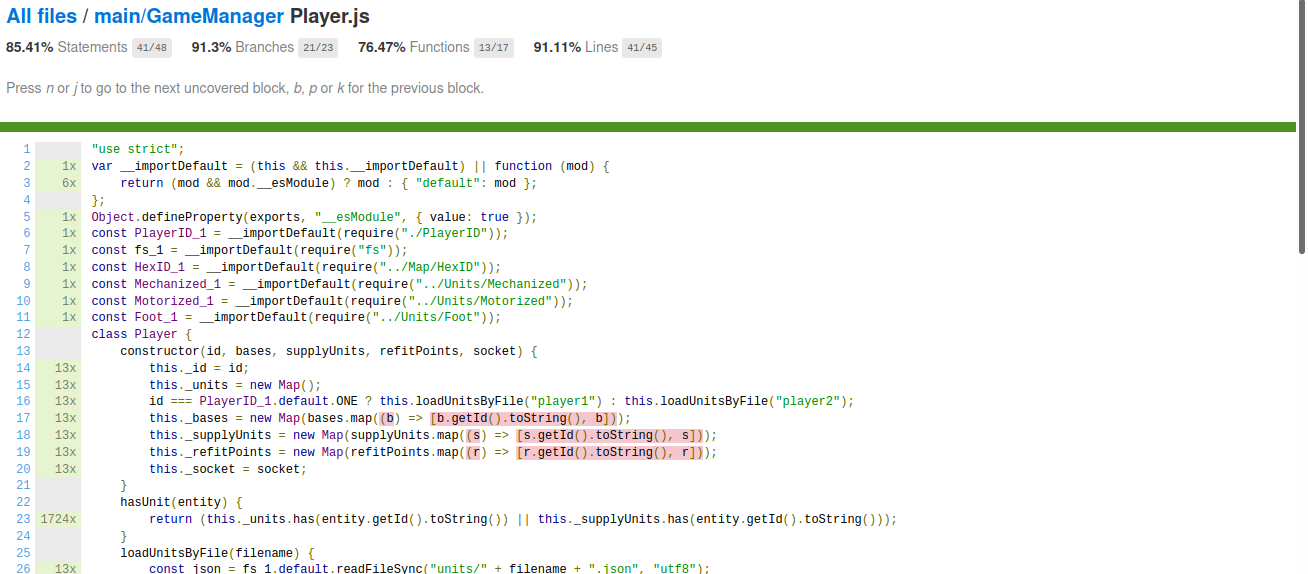
\includegraphics[scale=0.3]{data/couverture_test_2.png}
    \caption{Couverture d'un fichier}
\end{figure}

La couverture du code n'implique pas des tests de qualité. Après quelques recherches nous avons trouvé qu'une couverture minimale de bonne qualité dépasse les 80\%. Nous nous sommes donc fixés d'au moins atteindre ce pourcentage.